\chapter{QUADRO TEÓRICO}

\par Neste capítulo serão listados os conceitos e as tecnologias que serão
utilizados no desenvolvimento da proposta de trabalho apontada na seção 
objetivos. Para tal, serão discutidos a definição, o histórico e as 
aplicabilidades de cada um deles, tomando por base autores fundantes e 
seus comentaristas. É importante ressaltar que o texto desta seção, quando
descreve a teoria da evolução das espécies, não tem como objetivo levantar
questões sobre a origem dos seres vivos.

\section{Algoritmos Genéticos}

\par Nesta seção será descrito como surgiu, conceitos e algumas características
dos Algoritmos Genéticos, tema principal deste trabalho e fundamental para o
desenvolvimento da aplicação.

\subsection{Fundamentos}

\par Para \citeonline{livro_introduction_ag_melaine_mitchell}, desde o começo da
era computacional, cientistas pioneiros, tais como Alan Turing, John von
Neumann, Norbert Wiener e outros, tinham o objetivo de dotar os computadores de inteligência
de maneira que eles pudessem tomar decisões, se adaptar a determinadas situações
e até mesmo ter a capacidade de aprender. Com esta motivação, estes cientistas
se interessaram por outras áreas, além da eletrônica, como  a
biologia e a psicologia, e começaram então a realizar pesquisas para simular os
sistemas naturais no mundo computacional a fim de alcançarem suas metas. 

\par Vários conceitos computacionais baseados na natureza surgiram então ao
longo do tempo, dentre eles, a computação evolucionária inspirada na teoria da
evolução natural, da qual o exemplo mais proeminente são os AGs que foram
introduzidos por Jhon Holland, seu aluno David Goldberg e outros estudantes da universidade de Michigan.
\citeonline{livro_genetic_algorithm_goldberg} define os AGs como métodos de busca baseados na
genética e no mecanismo de seleção natural que permitem a possibilidade de obter
robustez e eficácia na tarefa de encontrar uma boa solução para um problema
em um espaço de busca complexo, em um tempo aceitável.


\par Segundo \citeonline{livro_ags_ricardo_linden}, a teoria da evolução foi proposta pelo naturalista
inglês Charles Darwin por volta de 1850, quando este, em uma viagem de navio
visitou vários lugares e por ser uma pessoa com uma grande habilidade de  observação, percebeu que indivíduos de uma mesma espécie vivendo em lugares diferentes possuíam também
características distintas, ou seja, cada indivíduo  possuía atributos
específicos que lhe permitia uma melhor adaptação em seu ecossistema. 


\par O autor afirma então que, com base nesta observação, Darwin propôs que existe um processo de
seleção natural, afirmando que, como os recursos na natureza, tais como água e comida,
são limitados, os indivíduos competem entre si e aqueles que não possuem atributos necessários
à adaptação ao seu ambiente tendem a ter uma probabilidade menor de reprodução e
irão ser extintos ao longo do tempo e, por outro lado, aqueles
com características que os permitem obter vantagens competitivas no meio onde
vivem, acabam tendo mais chances de sobreviver e gerar indivíduos ainda mais
adaptados. 

\par A teoria ressalta porém que o processo não tem o objetivo de maximizar
algumas características das espécies, pois  os novos indivíduos
possuem atributos que são resultados da mesclagem das características dos reprodutores,
o que faz com que os filhos não sejam exatamente iguais aos pais, podendo assim
ser superiores, uma vez que, estes herdem as qualidades de seus pais ou
inferiores se os descendentes herdarem as partes ruins de seus
reprodutores \cite{livro_ags_ricardo_linden}.

\par Para entender a relação entre AGs e a evolução natural é
necessário conhecer as principais terminologias biológicas, 
sendo importante ressaltar porém que, de acordo com
\citeonline{livro_introduction_ag_melaine_mitchell}, apesar da 
analogia a certos termos da biologia, a forma com que os AGs 
são implementados é relativamente simples se comparado ao funcionamento
biológico real.

\par \citeonline{livro_introduction_ag_melaine_mitchell} afirma que 
todos os seres vivos são compostos de células e estas possuem um ou mais
cromossomos que, basicamente, são manuais de instruções que definem as 
características do organismo. O cromossomo é formado por um conjunto de genes
que, em grupo ou individualmente, são responsáveis por um determinado atributo
do indivíduo como por exemplo, a cor do cabelo, a altura, etc. Cada gene possui
uma localização dentro do cromossomo denominada \textit{locus} e, por fim, o
conjunto de todos os cromossomos dentro da célula é definido como genoma. 

\par Considerando isto, \citeonline[p.33]{livro_ags_ricardo_linden} afirma que,

\begin{citacao}
	Um conjunto específico de genes no genoma é chamado de genótipo. O
	genótipo é a base do fenótipo, que é a expressão das características
	físicas e mentais codificadas pelos genes e modificadas pelo
	ambiente, tais como cor dos olhos, inteligência etc. Daí, podemos concluir: nosso
	DNA codifica toda a informação necessária para nos descrever, mas esta
	informação está sob controle de uma grande rede de regulação gênica
	que, associada às condições ambientais, gera as proteínas na quantidade
	certa, que farão de nós tudo aquilo que efetivamente
	somos.
\end{citacao}  

\par Uma vez descrita a complexidade dos organismos é necessário discorrer,
de forma básica, sobre o processo de reprodução responsável pela
transmissão da informação genética de geração para geração.

\par \citeonline{livro_ags_ricardo_linden} afirma que existem dois tipos de reprodução,
a assexuada, em que não é necessário a presença de um parceiro e a sexuada que exige a
presença de dois organismos.
Os AGs simulam a reprodução sexuada em que cada um dos organismos envolvidos
oferece um material genético denominado gametas. Os gametas são formados por um
processo denominado \textit{crossing-over} ou \textit{crossover} que tem início com a divisão de cada cromossomo em duas parte as quais 
irão se cruzar uma com a outra para formar dois novos cromossomos, que
receberão um pedaço de cada uma das partes envolvidas no cruzamento.

\par Ainda segundo o autor, o resultado deste processo serão, então, quatro
cromossomos potencialmente diferentes que irão compor os gametas e farão parte
dos novos indivíduos. Neste processo, podem ocorrer mutações que são resultados
de alguns erros ou da influência de algum fator externo, como a radiação por exemplo. Estas mutações são
pequenas mudanças nos genes dos indivíduos, podendo estas ser boas, ruins ou neutras.


\par E assim a informação genética é passada dos pais para os filhos, e como os
componentes dos cromossomos definem as características do organismo, os filhos
herdarão características dos pais, porém serão ligeiramente diferente deles,
como foi descrito anteriormente, o que permite que os novos indivíduos herdem
características melhores ou piores que seus progenitores, porém, se os pais
possuem características positivas, a probabilidade de gerarem filhos ainda
melhores são maiores \cite{livro_ags_ricardo_linden}.

\subsection{Características dos Algoritmos Genéticos}

\par De acordo com \citeonline{livro_ags_ricardo_linden}, a analogia dos AGs com
os processos biológicos se dá por meio da representação de cada termo descrito
anteriormente em um modelo computacional voltado a encontrar soluções para um
determinado problema em um processo aleatório. O fluxo de execução deste processo
inicia-se com a criação aleatória de uma população inicial. Uma população contém
um conjunto de indivíduos sendo que cada indivíduo  representa uma possível solução
para o problema.

\par O autor afirma ainda que um indivíduo é formado por cromossomos que
guardam as características da solução, ou seja, uma forma de resolver o
problema.

\par Segundo \citeonline{livro_introduction_ag_melaine_mitchell}, a execução de um 
algoritmo genético é basicamente realizada conforme os itens a seguir:

\begin{enumerate}
	\item Definição da população inicial;
	\item Avaliação e classificação dos indivíduos da população;
	\item Seleção de acordo com a qualidade;
	\item Cruzamento para geração de novos descendentes;
	\item Mutação aleatória dos novos indivíduos;
	\item Repetição do processo de seleção, cruzamento e mutação até se formar uma nova população;
	\item Avaliação e classificação dos indivíduos da nova população;
	\item A nova população substitui a anterior e o processo continua a partir do
	intem 2 até que o número de populações criadas atinja um limite, que é definido
	previamente, ou até atingir outra condição definida pelo programador.
\end{enumerate}

\par A Figura ~\ref{fig:representacao_ags} ilustra os passos do algoritmo.


\begin{figure}[h!]
	\centerline{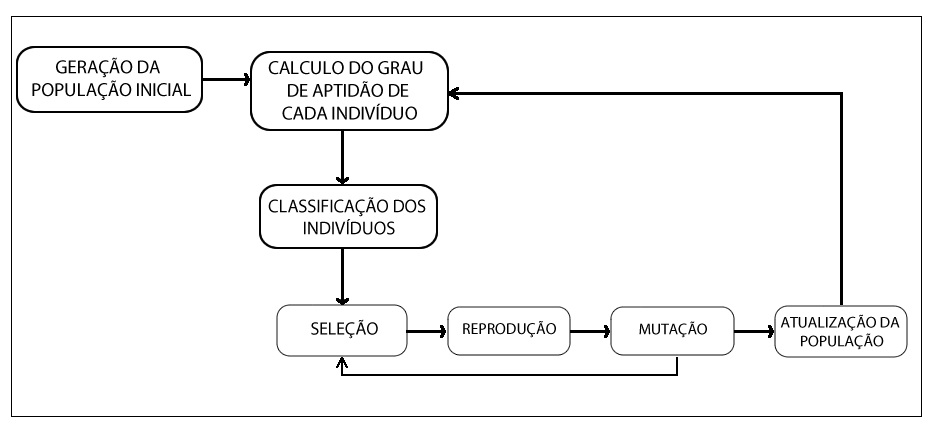
\includegraphics[scale=0.6]{./imagens/algoritimos_geneticos.jpg}}
	\caption[Demonstração da execução de um AG]
	{Demonstração da execução de um AG \textbf{Fonte:} Desenvolvido pelos autores.}
	\label{fig:representacao_ags}
\end{figure}

\par Como demostrado acima existem dois \texttt{loops}, o
\texttt{loop} que acontece até que uma nova população seja formada e outro
responsável por  iniciar a criação de uma nova população até que o
número de gerações seja atingido.

\subsubsection{População Inicial}

\par De acordo com \citeonline{livro_introduction_ag_melaine_mitchell}, a população inicial 
é o conjunto dos primeiros indivíduos candidatos à resolução do problema. Estes
indivíduos devem ser criados aleatoriamente, seguindo a lógica definida pelo programador com base no contexto do 
problema a ser resolvido. Um exemplo seria a população inicial do algoritmo desenvolvido neste trabalho, 
em que a população inicial será formada por possíveis formas de se produzir um determinado lote de calças, 
ou seja, será formada uma população de possíveis formas de dividir o trabalho entre as costureiras.

\subsubsection{Função de avaliação}

\par Segundo \citeonline{livro_ags_ricardo_linden}, após a criação da população
inicial, esta é então avaliada através de uma função de avaliação que mede a
qualidade de cada uma de suas soluções e é realizada então uma classificação que ordena as soluções das melhores para as
piores, para então iniciar a formação de uma nova população, a nova população
pode conter, já inicialmente, os dois melhores indivíduos existentes na
população inicial, este mecanismo é denominado elitismo e pode ser utilizado ou
não.

\par Ainda segundo o autor, a função de avaliação ou função de aptidão penaliza
as soluções inviáveis para a solução do problema, ou seja, ao verificar que uma
certa solução não satisfaz o grau de aptidão necessário para o problema
proposto, esta solução é descartada e, assim, só sobrevivem as soluções com mais
chance de resolver o problema e por isso torna-se o componente mais importante de qualquer algoritmo genético.

\par Devido à generalidade encontrada nos AGs, a função de avaliação
torna-se em muitos casos a única ligação verdadeira entre o programa e o
problema real pois ela irá analisar os cromossomos de cada indivíduo,
convertendo-os assim, em uma proposta de solução para o problema
\cite{livro_ags_ricardo_linden}.

% \par Baseando nessas \citeonline{livro_ags_ricardo_linden}, iremos
% usar no projeto uma função para avaliar dentre varias costureiras a melhor forma de
% destribuir a materia prima para que seja produzida uma certa quantidade de
% calças no menor tempo possível.


\subsubsection{Seleção}

\par Segundo \citeonline{livro_ags_ricardo_linden}, o próximo passo
para a formação da nova população é o cruzamento, que se inicia com a seleção de
dois indivíduos, que é realizada de acordo com a qualidade destes, porém,
como é fundamental que esta escolha não despreze completamente os indivíduos com uma
qualidade muito baixa, a seleção é feita de forma probabilística, ou seja,
indivíduos com boa qualidade possuem mais chances de serem selecionados e, por
outro lado, indivíduos com menor nota de avaliação terão menos chance se
reproduzirem.

\par O autor ressalta que a razão de o mecanismo de seleção não
escolher apenas as melhores soluções é devido ao fato de que aquelas com menor
grau de avaliação, também serem importantes para que se tenha uma maior diversidade de características
na população envolvida para a solução do problema, possibilitando assim
que esta possa evoluir de forma satisfatória, pois se as novas populações forem constituídas
somente das melhores soluções, elas serão compostas de indivíduos cada vez mais semelhantes
impedindo assim que novas soluções ainda melhores sejam concebidas.

\par Existem vários tipos de seleção. Um dos métodos utilizado para este fim é o método
roleta, muito utilizado entre a maioria dos pesquisadores de AGs. Metaforicamente, 
cada indivíduo da população ocupa uma porção da roleta, proporcional ao seu índice 
de aptidão, ou seja, os indivíduos que possuírem maior aptidão ocuparão uma maior 
porção do que aqueles com menor aptidão. A roleta, então, assim como mostra a
Figura ~\ref{fig:metodo_selecao_roleta}, é girada e o indivíduo escolhido é
aquele em que a seta parar sobre ele \cite{REVISTA_MULTIDISCIPLINAR_DA_UNIESP}.


\begin{figure}[h!]
	\centerline{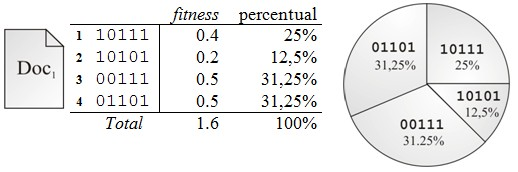
\includegraphics[scale=1.0]{./imagens/roleta.jpg}}
	\caption[Demonstração do método de seleção Roleta]
	{Demonstração do método de seleção Roleta \textbf{Fonte:}
	"http://www.dgz.org.br/fev09/Art04.htm".}
	\label{fig:metodo_selecao_roleta}
\end{figure}



\subsubsection{Cruzamento} 

\par Segundo \citeonline{livro_ags_ricardo_linden}, após a seleção dos pais, irá
ocorrer então o processo de cruzamento ou \textit{crossover} e, como no cruzamento natural, neste processo dois novos indivíduos, ou seja, duas
novas soluções são formadas a partir de características daquelas que se
cruzaram, ou seja, serão geradas duas novas soluções que conterão alguns cromossomos
de uma solução e alguns cromossomos de outra.

\par Para \citeonline{intro_aos_algoritimos_geneticos}, o operador
\textit{crossover} é um mecanismo de busca dos AGs para explorar regiões
desconhecidas do espaço de busca. Ele é aplicado a cada par de cromossomos dos
indivíduos que passaram pelo processo de seleção, gerando assim, dois novos
indivíduos.

\par Para \citeonline{REVISTA_MULTIDISCIPLINAR_DA_UNIESP}, o cruzamento combina
os cromossomos pais a fim de gerar cromossomos filhos e para isso existem vários
tipos de cruzamento.

\par Um dos cruzamentos muito utilizado é o cruzamento de um ponto, que divide a
lista de cromossomos selecionados em um ponto de sua cadeia, esse ponto é escolhido aleatoriamente.
Após essa divisão, é copiada uma parte dos cromossomos de cada pai para definir
os cromossomos dos indivíduos filhos. Neste método, é comum os pais gerarem dois
novos filhos \cite{REVISTA_MULTIDISCIPLINAR_DA_UNIESP}.

\par Um outro cruzamento muito utilizado é o cruzamento uniforme, que
ainda segundo o autor, gera cada gene do descendente copiando o gene em questão
de um dos pais, em que se usa uma máscara de cruzamento que é gerada aleatoriamente para fazer a escolha.
Para criar cada cromossomo do novo indivíduo é feita uma iteração em todas as
posições da máscara fazendo uma análise dos seus valores, quando o valor da posição for 1, o gene do
primeiro pai referente à mesma posição da máscara é copiado, se o valor for 0
será copiado o gene do segundo pai, depois desse processo é gerado o novo
descendente.

\par Segundo \citeonline{intro_aos_algoritimos_geneticos}, o tipo de cruzamento
uniforme difere do cruzamento de um ponto uma vez que este sempre leva à
metade dos \textit{bits} de cada pai.

\subsubsection{Mutação}

\par Para \citeonline{livro_ags_ricardo_linden}, também pode ocorrer a mutação em
que, como ocorre na natureza, aleatoriamente o valor dos
cromossomos de um indivíduo pode ser alterado. A mutação ocorre de acordo com
uma taxa definida. Basicamente é definida uma porcentagem baixa e então um
número de 0 a 1 é sorteado e multiplicado por 100, se o resultado for menor que
a porcentagem definida, irá ocorrer a mutação para aquele indivíduo.

\par Para \citeonline{intro_aos_algoritimos_geneticos}, a mutação melhora a
diversidade dos cromossomos na população. Em contrapartida, depois de realizada
a mutação se perdem as informações contidas no cromossomo. Assim, para assegurar
a diversidade deve-se usar uma taxa de mutação pequena. 


\par Assim como no cruzamento há vários tipos de mutação, dentre eles a mutação
de \textit{bit} que é um tipo de mutação mais simples de ser implementada.

\par Segundo \citeonline{REVISTA_MULTIDISCIPLINAR_DA_UNIESP} este é o operador
mais fácil de trabalhar podendo ser aplicado em qualquer forma de representação
binária dos cromossomos. Este tipo de mutação gera uma probabilidade de mutação
para cada \textit{bit} do cromossomo, caso a probabilidade sorteada estiver
dentro da taxa de mutação definida, o \textit{bit} sofrerá mutação, recebendo um
valor determinado de forma aleatória dentre os valores que podem ser assumidos pelo cromossomo.


\par No problema a ser solucionado na aplicação deste trabalho, há um
cenário em que existem diversas soluções para se resolver o problema e deseja-se
encontrar a melhor dentre elas. Conforme descrito anteriormente, os AGs são uma
das melhores opções para se resolver este tipo de problema, por este motivo esta técnica foi escolhida.

% \par Para \citeonline[p.4]{ifsudestemg}, a proposta da Orientação a
% Objetos é,
% 
% \begin{citacao}
% Representar o mais fielmente possível as
% situações do mundo real nos sistemas computacionais. Nós entendemos o mundo
% como um todo composto por vários objetos que interagem uns com os outros. Da
% mesma maneira, a Orientação a Objetos consiste em considerar os sistemas
% computacionais não como uma coleção estruturada de processos, mas sim como
% uma coleção de objetos que interagem entre si.
% \end{citacao}  


% 
% Este processo é iniciado com um conjunto de várias soluções
% candidatas que fazem alusão aos cromossomos e cada solução possui atributos que
% definem como o problema pode ser resolvido. Tais atributos fazem alusão aos
% genes e os valores que estes atributos podem assumir, seja um valor numérico,
% ou um texto, por exemplo, fazem referência aos alelos. Após estas definições 
% durante a execução do algoritmo, ocorre o processo de reprodução em que as
% soluções se cruzam entre si, simulando o processo de \textit{crossing-over} no
% intuito de gerarem soluções possivelmente melhores, alem disto também é simulado
% o processo de mutação em que aleatóriamente um atributo de uma solução pode ser alterado.
% No final deste processo existe um mecanismo que mede a qualidade das soluções
% geradas e o processo continua até que a melhor solução seja encontrada ou até que o número
% de reproduções, definido préviamente, seja atingido, neste caso a melhor solução
% encontrada até aquele momento será o resultado do processo, ou seja, a melhor
% solução naquela execução, sendo importante ressaltar porém que outras execuções
% podem gerar resultados diferentes. \cite{livro_introduction_ag_melaine_mitchell}


\section{Tecnologias}

\par Abaixo serão listadas as tecnologias que serão utilizadas no
desenvolvimento do projeto.

\subsection{Linguagem de programação Java}

\par Segundo \citeonline{oracle}, a Linguagem Java foi projetada
para permitir o desenvolvimento de aplicações seguras, portáteis
e de alto desempenho para a mais ampla gama de plataformas de computação.

\par De acordo com \citeonline{livro_java_complete_references}, o Java foi
criado em 1991 pela \textit{Sun Microsystems} e foi baseado em uma linguagem já
existente, o C++, que foi escolhida por ser orientada a objetos e
por gerar códigos compactados, o que era exatamente o que eles precisavam para
implantar em pequenos aparelhos. Além dessas características, um requisito
desejável era que a nova linguagem fosse independente de plataforma, para que
fosse executado em qualquer arquitetura, tais como, TVs, telefones, entre
outros, e então, para atender esta exigência, foi
criado o conceito de máquina virtual, que ficou conhecido como \textit{Java
Virtual Machine} - JVM\footnotemark[2].

\footnotetext[2]{O termo Java Virtual Machine será referenciado pela sigla JVM a
partir deste ponto do trabalho.}

\par O ponto chave que
permite o Java resolver o problema de portabilidade é o fato de o código ser
compilado em \textit{Bytecode}, que é um conjunto genérico de instruções
altamente otimizado que é executado pela JVM, e esta, por sua vez, traduz o
mesmo para a arquitetura a qual ela está instalada o que possibilita a execução do programa
em várias plataformas \cite{livro_java_complete_references}.
%Ver este contexto resolvendo assim também problemas associados com programas baseados na web. 


% 
% \par Hoje os Browsers que possuem JVM embutida podem executar programas que 
% utilizam a linguagem JAVA. 
% 
% Neste particular Quinteiro (2006) registrou que:
% 
% \begin{citacao}
% “A Sun considera o sucesso do Java na Internet como sendo o primeiro passo para utilizá-lo em decodificadores da 
% televisão interativa, em dispositivos portáteis e outros produtos eletrônicos de consumo - exatamente como o Java 
% tinha começado em 1991. Sua natureza portátil e o projeto robusto permitem o desenvolvimento para múltiplas 
% plataformas, em ambientes tão exigentes como os da eletrônica de consumo".\cite[p.33]{livro_ags_ricardo_linden}
% \end{citacao}  


\par Além da portabilidade, o Java também é \textit{multithread}, ou seja,
permite a execução de múltiplas tarefas simultaneamente. A linguagem também
conta com um \textit{automatic garbage collector} que consiste em um mecanismo
de gerenciamento e limpeza de memória que a JVM acomoda. Além disso o Java
suporta uma extensa biblioteca de rotinas que facilitam a interação com protocolos 
TCP/IP, como HTTP e FTP \cite{livro_java_complete_references}.

\par De acordo com \citeonline{livro_java_Guia_do_Programador}, 

\begin{citacao} Atualmente a linguagem está organizada em três segmentos
principais:


	- JavaMe (\textit{Java Micro Edition}) - Destinado a pequenos dispositivos
	computacionais móveis, tais como celulares, PDAs e \textit{set-top boxes}. É
	composto de máquina virtual otimizada para ambientes mais restritos, com
	especificações de funcionalidades e uma API mais compacta;
	  
	- JavaSE (\textit{Java Standard Edition}) - Integra os elementos padrão
	da plataforma e permite o desenvolvimento de aplicações de pequeno e médio porte. Inclui todas as APIs consideradas de base,
além da máquina virtual padrão;

	- JavaEE (\textit{Java Enterprise Edition}) - Voltada para o desenvolvimento
	de aplicações corporativas complexas. Adiciona APIs específicas aos elementos
	padrão da plataforma.
	

\end{citacao}


\par Para \citeonline{livro_intro_a_prog_orientada_objetos_usando_java}, Java é
uma linguagem Orientada a Objetos (OO), este paradigma usa objetos, criados a
partir de modelos, também chamados de classes, para representar e processar
dados em aplicações computacionais. Basicamente uma classe ou modelo é um
conjunto de especificações de um objeto, ou seja, que tipo de dados este deve
ter e quais operações este terá e então após a criação da classe o programador
pode criar um objeto desta. Uma analogia simples seria a planta de uma casa e a
construção da mesma em si, a planta representa a classe, ou seja, como a casa deve ser feita e a casa depois de construída representa o objeto.

\par Os dados e operações são guardados em objetos e estes são os elementos
centrais do programa. Assim a aplicação como um todo é vista como uma coletânea
de objetos que se relacionam uns com os outros. Cada objeto representa um conceito real de uma parte do problema. 
Isto permite que o desenvolvimento se torne menos complexo pois os conceitos são familiares
às pessoas envolvidas no projeto pelo fato de que a aplicação não está
organizada em processos estruturados mas sim em objetos que espelham o mundo real e interagem entre si  \cite{teste_doutorado_manzoni}.

\par Para \citeonline{livro_intro_a_prog_orientada_objetos_usando_java}, 
os dados pertencentes aos modelos são representados por tipos nativos,
característicos das linguagem de programação e podem também ser representados
por outros modelos criados pelo programador.

%\par O autor ainda exemplifica um modelo como a representação de um funcionário
% de uma empresa para fins de processamento de folha de pagamento. Neste caso o
%modelo representaria dentre outros dados, o nome, cargo, salário e horas extras
% trabalhadas dessa pessoa, e as operações seria aquelas relacionados com realização
% de cálculos de salário e impostos, por exemplo.

\par Para o desenvolvimento do sistema de informação deste projeto, o paradigma
de orientação a objetos, que será implementado na linguagem Java, será
imprescindível devido à alta complexidade do problema a ser resolvido. Pois cada objeto representará partes do algoritmo genético que será desenvolvido, tais
como a representação do Indivíduo, Cromossomos, etc, o que facilitará muito o
desenvolvimento.

\par O produto resultante deste trabalho faz uso do Java EE e, como já foi dito
em seções anteriores, será implementado em plataforma WEB. Para tal, faz-se
necessário o uso de um servidor de aplicações WEB. Dentre as opções disponíveis, foi escolhido o \textit{Tomcat} pelo fato de este ser o mais simples e ter os atributos mínimos necessários para a aplicação que
será desenvolvida.

\par Segundo \citeonline{livro_apache_tomcat_7}, o \textit{Tomcat} é um
servidor \textit{open source} e \textit{container} de aplicações \textit{web}
baseados em Java. Ele foi criado para executar \textit{servlets}, que também é
uma denominação para classe dentro da especificação do Java para WEB, e arquivos
de marcação que definem os elementos visuais da tela que será explanado na seção.
O \textit{Tomcat} foi criado como um subprojeto da \textit{Apache-Jakarta}, porém como ficou
muito popular entre os desenvolvedores, a \textit{Apache} o denominou como um
projeto separado e vem sendo melhorado e apoiado por um grupo de voluntários da comunidade \textit{Java Open Source}, que o faz 
uma excelente solução para desenvolvimento de uma aplicação \textit{web} completa. 

 

\subsection{Interface Gráfica - JSF}


\par Para a construção da interface gráfica (páginas web) da aplicação
desenvolvida neste trabalho, foi utilizado um \textit{framework} nativo nas
novas versões do Java denominado \textit{Java Server Faces} (JSF).

\par \citeonline{bergsten_javaserver_faces} afirma que o JSF é um
\textit{framework server-side} baseado em componentes \textit{web}, cuja principal função é abstrair os detalhes de manipulação dos eventos e organização dos componentes na página \textit{web}. 
Por meio dele, é possível desenvolver páginas mais sofisticadas de forma
simples, abstraindo, inclusive, o tratamento de requisições e respostas. Isto permite ao desenvolvedor focar-se no \textit{back-end} da aplicação, ou seja, na lógica, e não se preocupar com detalhes a respeito de requisições e respostas HTTP e como obter as informações recebidas e/ou enviadas através deste protocolo.

\par De acordo com \citeonline{oracle_javaserver_faces_technology_overview}, o
JSF é de fácil aprendizado e utilização, pois possui sua arquitetura claramente definida, sendo dividida entre a lógica da aplicação e apresentação. Esta divisão é possível pois ele utiliza o padrão de projeto \textit{Model-View-Controller} - MVC\footnotemark[3], tornando-o um importante \textit{framework} para desenvolvimento de aplicações utilizando a plataforma Java \textit{Web}.

\footnotetext[3]{MVC: \textit{Model-View-Controller} - \textit{Design
pattern}, padrão de arquitetura de software que separa a informação (e as suas
regras de negócio) da interface com a qual o usuário interage.}

%BANCA_QUALIFICACAO. Comentado este parágrafo, porém o mesmo retornará para a banca de qualificação
\par Segundo
\citeonline{gamma_helm_johnson_vlissides_design_patterns_elements_reusable_object_oriented_software}, 
o padrão de projeto MVC é dividido em três partes. O \textit{Model} é a lógica e
acesso aos dados da aplicação, a \textit{View} é camada de apresentação e por
último o \textit{Controller} é responsável por definir a interface entre a lógica e a apresentação. Portanto, todo tipo de requisição ou resposta deve ser obrigatoriamente enviada 
ao \textit{Controller}, que, por sua vez encaminhará para a camada de visão ou
de lógica. A Figura ~\ref{fig:modelo_mvc} demonstra um exemplo do modelo MVC
utilizando o JSF.

% Imagem do modelo MVC usando JSF - VOLTAR PARA A BANCA DE QUALIFICACAO
\begin{figure}[h!]
	\centerline{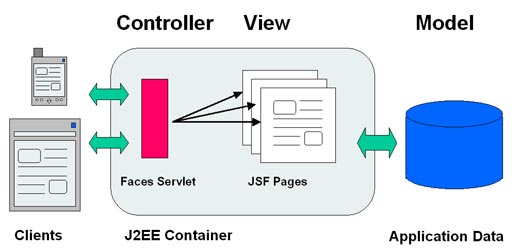
\includegraphics[scale=0.5]{./imagens/jsf_using_mvc.jpg}}
	\caption[Demonstração do Modelo MVC]
	{Demonstração do Modelo MVC. \textbf{Fonte:}
	http://www.javabeat.net/jsf-2/.}
	\label{fig:modelo_mvc}
\end{figure}

%BANCA_QUALIFICACAO. Comentado este parágrafo, porém o mesmo retornará para a banca de qualificação
\par Ao utilizar o JSF, toda e qualquer interação que o usuário realizar com a aplicação será executada por 
um \textit{servlet} chamado \textit{Faces Servlet}. Ele é a responsável por
receber tais requisições da camada de visão e redirecioná-las à lógica da aplicação e, posteriormente, enviar a resposta ao 
usuário \cite{faria_java_ee_7_jsf_primefaces_cdi}.

\par Segundo \citeonline{livro_programacao_java_para_web}, a especificação do \textit{JavaServer
	Faces} foi definida pela \textit{Java Comunity Process} - JCP\footnotemark[4],
	que é uma entidade cujo objetivo é especificar a evolução do Java. E por este motivo grandes empresas como
\textit{Apache}, \textit{IBM}, \textit{Oracle}, entre outras, participaram
desta definição. As implementações mais conhecidas são da especificação do JSF são:

\footnotetext[4]{O termo \textit{Java Comunity Process} será referenciado pela
	sigla JCP a partir deste ponto do trabalho.}

\begin{itemize}
	\item \textit{Sun Mojarra} (antes JSF R1) – implementação de referência
	(\url{http://javaserverfaces.java.net/})
	
	\item \textit{MyFaces} da \textit{Apache} (\url{http://myfaces.apache.org/})
\end{itemize}

\par Com essas implementações é possível utilizar todos os recursos do padrão JSF,
como formulários, tabelas, \textit{layout}, conversão e validação de eventos,
além de toda a inteligência para a interpretação dos arquivos de configuração e
interação com o \textit{container} Java. Como o JSF é um padrão de mercado,
várias empresas investem no desenvolvimento de bibliotecas de componentes como, calendário, barras de progresso, menus,
efeitos de transição entre outros \cite{livro_programacao_java_para_web}.

\par Algumas das principais bibliotecas de componentes são:

\begin{itemize}
	\item \textit{Trinidad}, da \textit{Apache MyFaces}
	(\url{http://myfaces.apache.org/trinidad/});
	
	\item \textit{Tobago}, da \textit{Apache MyFaces}
	(\url{http://myfaces.apache.org/tobago/});
	
	\item \textit{ICEFaces}, da \textit{ICESoft} (\url{http://www.icefaces.org/});
	
	\item \textit{RichFaces}, da \textit{JBoss}
	(\url{http://www.jboss.org/richfaces/});
	
	\item \textit{Tomahawk}, da \textit{Apache MyFaces}
	(\url{http://myfaces.apache.org/tomahawk/});
	
	\item \textit{PrimeFaces} (\url{http://www.primefaces.org/}).
\end{itemize}

\par Neste trabalho, é utilizada a biblioteca PrimeFaces, que é uma
biblioteca de componentes que implementa a especificação do JSF. Ele possui uma ampla gama de componentes disponíveis 
para auxiliar o desenvolvimento de interfaces \textit{web} ricas, além de possuir o seu
código fonte aberto \cite{ross_borsoi_uso_primefaces}.

\par Para \citeonline{juneau_primefaces_enterprise}, uma das grandes vantagens
do Primefaces é a facilidade de integração entre ele e o JSF, bastando apenas
incluir a biblioteca do Primefaces no projeto JSF, salvo alguns componentes
específicos, como o \textit{file upload}, que necessita de pequenas configurações adicionais.
Essas mudanças, quando necessárias, devem ser realizadas no arquivo de
configuração da aplicação que, por padrão, é chamado de \textit{web.xml}, porém,
o mesmo pode ser alterado pelo desenvolvedor.

\par Por possuir as vantagens descritas acima e uma simples configuração, além de ser um 
\textit{framework cross-browser\footnotemark[5]}, o JSF foi escolhido para
auxiliar no desenvolvimento das páginas \textit{web} deste trabalho.

% E por todas as vantagens do Primefaces mencionadas, somado ao fato de esta
% biblioteca possuir uma ótima documentação em conjunto com uma grande comunidade de desenvolvedores que a 
% utilizam e a alta demanda de desenvolvedores que a conhecem no mercado, ela foi
% escolhida em conjunto com o JSF para desenvolvimento das páginas \textit{web}
% deste trabalho.

\footnotetext[5]{\textit{Cross-Browser} - Compatibilidade com todos os tipos de
dispositivos e navegadores}

% \par O \textit{Apache Tomcat} é um servidor web estável, ele 
% possui varias funcionalidades como o \textit{Tomcat Manager},
% \textit{Specialized Realm Implementations} e \textit{Tomcat Valves}. O
% \textit{Tomcat Manager} é fornecido com o servidor \textit{Tomcat} e é
% responsável pela funcionalidade básica para gerenciar aplicações web em execução no servidor \textit{Tomcat} 
% a partir de qualquer navegador. Ja o \textit{Specialized Realm Implementations}
% é um método de segurança que o Tomcat disponibiliza para proteger os recursos
% dentro do \textit{container} que é um recipiente que funciona como um banco de
% dados de usuários e esses bancos são denominados \textit{Realm}. O
% \textit{Tomcat Valves} é uma tecnologia que foi introduzido no Tomcat 4 e esta disponível nas versões
% posteriores e permitem associar instâncias de uma classe JAVA com um
% \textit{container} \textit{Catalina} particular, agindo como um pré-processador
% para todos os pedidos que vêm para o \textit{container}. 
% \cite{livro_apache_tomcat_7}



%\par Segundo a Apache (2015), o Tomcat é um software livre que realiza a
%implementação de especificações do Java voltado para programação para 
%internet lançado pela própria Apache.
% \par Exemplo de parágrafo utilizando comando para formatar em itálico as palavras em inglês, como por exemplo: \textit{pets, animals and software} e um exemplo de texto em negrigo: \textbf{grafo}.
% 
% \par Um tipo de citação: segundo \citeonline{correa2003plantas} as plantas \ldots.
% 
% \par Outro tipo de citação: as plantas \ldots \cite{correa2003plantas}.
% 
% \par Outro tipo de citação com página: \cite[p. 13]{correa2003plantas}.
% \par Outro tipo ainda de citação com página:  \citeonline[p. 13]{correa2003plantas}.
% 
% \par Para referenciar seções e capítulos, é necessário colocar o \textbackslash label e a referência assim: na \autoref{sec:materiais} e no \autoref{cap:quadroMetodologico} são encontradas as informações\ldots
% 
% \par Exemplo de equação:
% 
% \begin{equation}
%  \Delta Q = 
%  \left[
%  \frac{\sum_{in} + k_{i,in}}{2m} - 
%  \left(
%  \frac{\sum_{tot} + k_i}{2m}
%  \right)^2
%  \right] -
%  \left[
%  \frac{\sum_{in}}{2m} - 
%  \left(\frac{\sum_{tot}}{2m}
%  \right)^2 - 
%  \left(\frac{k_i}{2m}
%  \right)^2
%  \right]
% \end{equation}
% 
% 
% \par Símbolos matemáticos só funcionam dentro do ambiente \texttt{equation} ou entre dois símbolos \$. Ex: Adiciona cada vértice $w \in N_d(v) \Delta \Gamma$ na região, os quais foram vistos por pelo menos a uma fração $\gamma$ dos vértices em $N_d(v)$.
% 
% \par Outra fórmula: $y=x^2$
% 
% \section{Materiais}
% \label{sec:materiais}
% 
% \par Este parágrafo mostra um exemplo de um teste de nota de rodapé, utilizando o texto do documento da Univas\footnote{O nome “Desenvolvimento” é muito vago, portanto, não o utilize; prefira, de acordo com a situação, ``Fundamentação teórica'', ``Análise dos dados'', ``Objetivos'', ``Metodologia'', etc. }. Outro tipo de nota de rodapé\footnote{\cite{correa2003plantas}}.  Outro tipo ainda de nota de rodapé\footnote{\citeonline{correa2003plantas}}
% 
% 
% \par Um exemplo de tabela é mostrado na Tabela~\ref{tab:informativa}
% 
% 
% \begin{table} [h]
%   \caption[Informação nutricioal dos alimentos]
%           {Informação nutricioal dos alimentos \textbf{Fonte:} \cite{correa2003plantas}}
%   \centering
%   \begin{tabular}{|p{0.7in}|p{2in}|p{3in}|}
%     \hline 
%     \multicolumn{1}{|c|}{\textbf{Hortaliça}} & \multicolumn{1}{c|}{\textbf{Valor Nutricional}} & \multicolumn{1}{c|}{\textbf{Propriedades medicinais}} \\
%     \hline 
% Tomate
% &Vitamina A, C, E e ferro, potássio
% &Maior resistência aos vasos sanguíneos, combate a infecções\\
%     \hline 
% Cenoura
% &Vitamina A, vitaminas do complexo B, cálcio, fósforo
% &Regula o aparelho digestivo, purifica a bile e fortalece a pele\\
%     \hline
% Cebolinha
% &Cálcio, ferro, niacina
% &Estimula o apetite, ajuda na formação de ossos e dentes\\
% 
%     \hline
% Alface
% &Ferro, cálcio, niacina, vita\-mina C
% &Combate insônia, ajuda na cicatrização dos tecidos\\
% 
%     \hline
% Rúcula
% &Iodo, vitaminas A e C
% &Combate a fadiga, depura o sangue\\
% 
%     \hline
% Erva cidreira
% &Sais minerais
% &Tonico nervoso, combate cólicas intestinais\\
% 
%     \hline 
%   \end{tabular}
%   \legend{Fonte: \cite{correa2003plantas}}
%   \label{tab:informativa}
% \end{table}
% 
% \par A seguir segue exemplo de listagem numérica:
% 
% \begin{enumerate}
%   \item conteúdo do item 1;
%   \item conteúdo do item 2;
%   \item conteúdo do item 3;
%   \item conteúdo do item 4;
%   \item conteúdo do item 5;
%   \item conteúdo do item 6;
%   \item etc.
% \end{enumerate}
% 
% \par Também é possível fazer a lista de itens:
% 
% \begin{itemize}
%   \item conteúdo do primeiro item;
%   \item conteúdo do segundo item;
%   \item conteúdo do terceiro item;
%   \item conteúdo do quarto item;
%   \item conteúdo do quinto item;
%   \item etc.
% \end{itemize}
% 
% \par Um exemplo de imagem é mostrado na Figura~\ref{fig:exemplo1}.
% 
% \begin{figure}[h!]
%   \centerline{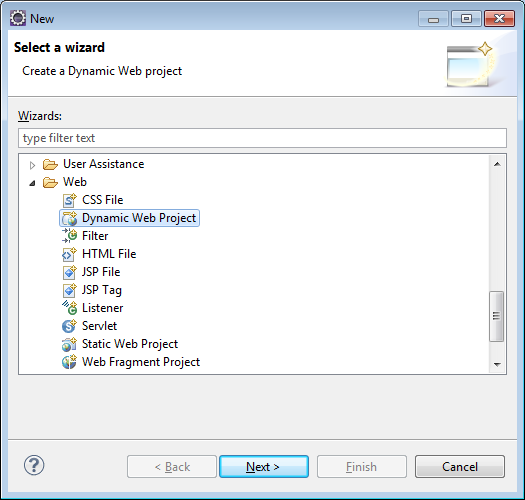
\includegraphics[scale=0.65]{./imagens/apendice_img1.png}}
%   \caption[Exemplo de criação de um projeto Web no Eclipse]
%           {Exemplo de criação de um projeto Web no Eclipse. \textbf{Fonte:} \cite{correa2003plantas}}
% \label{fig:exemplo1}
% \end{figure}
% 
% \par Perceba que o \LaTeX~faz a numeração automática das figuras e já adiciona na lista de figuras.
% 
% \par Agora a mesma imagem foi incluída, porém em escala menhor, conforme ilustra a Figura~\ref{fig:exemplo2}.:
% 
% \begin{figure}[h!]
%   \centerline{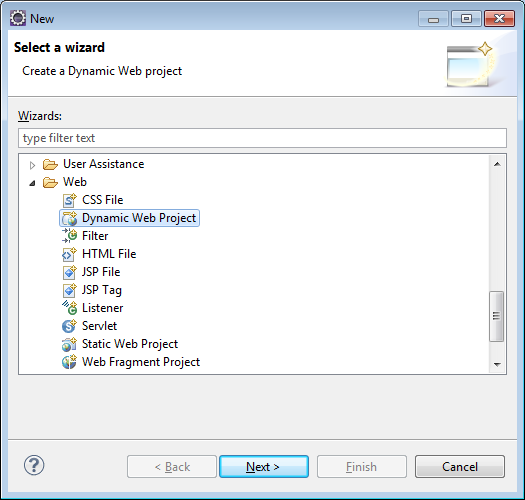
\includegraphics[scale=0.25]{./imagens/apendice_img1.png}}
%   \caption[Mesma imagem em escala menor]
%           {Mesma imagem em escala menor. \textbf{Fonte:} \cite{correa2003plantas}}
% \label{fig:exemplo2}
%\end{figure}


\subsection{Armazenamento de dados}

\par A aplicação desenvolvida neste trabalho irá demandar o armazenamento de
informações das costureiras e da disponibilidade das mesmas. Além disso, as saídas
oferecidas pelo algoritmo genético deverão ser armazenadas para uso posterior,
alimentando, assim, a base de dados do sistema, fazendo-se necessário o
uso de um banco de dados.

\par O gerenciador de banco de dados a ser utilizado nesta aplicação é o PostgreSQL, que 
foi escolhido por ser uma ferramenta robusta e \textit{open source}. O
PostgreSQL é um banco de dados relacional desenvolvido pela universidade da California por volta de 1970. Na
época, o projeto se chamava Ingres e só passou a se chamar Postgres por volta de 1986 quando Michael Stonebraker adicionou
o conceito de orientação a objetos ao projeto e decidiu então definir um novo
nome para a nova versão \cite{livro_postgres_doulgas}.

\par Para \citeonline{livro_introd_sistemas_bd} , ``um banco de dados é um
sistema computadorizado cuja funcionalidade geral é armazenar informações e
permitir que os usuários busquem e atualizem essas informações quando as
solicitar''. Já o conceito de banco de dados relacional é definido por
\citeonline[p.30]{oracle_database_sql} como:
\begin{citacao}
uma coleção de informações relacionadas, organizadas em tabelas. Cada tabela
armazena dados em linhas; os dados são organizados em colunas. As tabelas são
armazenadas em esquemas de banco de dados, que são áreas  onde os usuários 
podem armazenar suas próprias tabelas.
\end{citacao}
 \par Para manipular e acessar as informações em um banco de dados relacional
 é usada uma linguagem denominada SQL (\textit{Structured Query Language}), que
 foi projetada  especificamente para este fim. A linguagem foi desenvolvida
 pela IBM por volta de 1970 que tomou como base o trabalho do Dr. Edgar Frank
 Codd e possui uma sintaxe simples de fácil aprendizado e utilização \cite{oracle_database_sql}.


%\par Segundo a Apache (2015), o Tomcat é um software livre que realiza a
%implementação de especificações do Java voltado para programação para 
%internet lançado pela própria Apache.
% \par Exemplo de parágrafo utilizando comando para formatar em itálico as palavras em inglês, como por exemplo: \textit{pets, animals and software} e um exemplo de texto em negrigo: \textbf{grafo}.
% 
% \par Um tipo de citação: segundo \citeonline{correa2003plantas} as plantas \ldots.
% 
% \par Outro tipo de citação: as plantas \ldots \cite{correa2003plantas}.
% 
% \par Outro tipo de citação com página: \cite[p. 13]{correa2003plantas}.
% \par Outro tipo ainda de citação com página:  \citeonline[p. 13]{correa2003plantas}.
% 
% \par Para referenciar seções e capítulos, é necessário colocar o \textbackslash label e a referência assim: na \autoref{sec:materiais} e no \autoref{cap:quadroMetodologico} são encontradas as informações\ldots
% 
% \par Exemplo de equação:
% 
% \begin{equation}
%  \Delta Q = 
%  \left[
%  \frac{\sum_{in} + k_{i,in}}{2m} - 
%  \left(
%  \frac{\sum_{tot} + k_i}{2m}
%  \right)^2
%  \right] -
%  \left[
%  \frac{\sum_{in}}{2m} - 
%  \left(\frac{\sum_{tot}}{2m}
%  \right)^2 - 
%  \left(\frac{k_i}{2m}
%  \right)^2
%  \right]
% \end{equation}
% 
% 
% \par Símbolos matemáticos só funcionam dentro do ambiente \texttt{equation} ou entre dois símbolos \$. Ex: Adiciona cada vértice $w \in N_d(v) \Delta \Gamma$ na região, os quais foram vistos por pelo menos a uma fração $\gamma$ dos vértices em $N_d(v)$.
% 
% \par Outra fórmula: $y=x^2$
% 
% \section{Materiais}
% \label{sec:materiais}
% 
% \par Este parágrafo mostra um exemplo de um teste de nota de rodapé, utilizando o texto do documento da Univas\footnote{O nome “Desenvolvimento” é muito vago, portanto, não o utilize; prefira, de acordo com a situação, ``Fundamentação teórica'', ``Análise dos dados'', ``Objetivos'', ``Metodologia'', etc. }. Outro tipo de nota de rodapé\footnote{\cite{correa2003plantas}}.  Outro tipo ainda de nota de rodapé\footnote{\citeonline{correa2003plantas}}
% 
% 
% \par Um exemplo de tabela é mostrado na Tabela~\ref{tab:informativa}
% 
% 
% \begin{table} [h]
%   \caption[Informação nutricioal dos alimentos]
%           {Informação nutricioal dos alimentos \textbf{Fonte:} \cite{correa2003plantas}}
%   \centering
%   \begin{tabular}{|p{0.7in}|p{2in}|p{3in}|}
%     \hline 
%     \multicolumn{1}{|c|}{\textbf{Hortaliça}} & \multicolumn{1}{c|}{\textbf{Valor Nutricional}} & \multicolumn{1}{c|}{\textbf{Propriedades medicinais}} \\
%     \hline 
% Tomate
% &Vitamina A, C, E e ferro, potássio
% &Maior resistência aos vasos sanguíneos, combate a infecções\\
%     \hline 
% Cenoura
% &Vitamina A, vitaminas do complexo B, cálcio, fósforo
% &Regula o aparelho digestivo, purifica a bile e fortalece a pele\\
%     \hline
% Cebolinha
% &Cálcio, ferro, niacina
% &Estimula o apetite, ajuda na formação de ossos e dentes\\
% 
%     \hline
% Alface
% &Ferro, cálcio, niacina, vita\-mina C
% &Combate insônia, ajuda na cicatrização dos tecidos\\
% 
%     \hline
% Rúcula
% &Iodo, vitaminas A e C
% &Combate a fadiga, depura o sangue\\
% 
%     \hline
% Erva cidreira
% &Sais minerais
% &Tonico nervoso, combate cólicas intestinais\\
% 
%     \hline 
%   \end{tabular}
%   \legend{Fonte: \cite{correa2003plantas}}
%   \label{tab:informativa}
% \end{table}
% 
% \par A seguir segue exemplo de listagem numérica:
% 
% \begin{enumerate}
%   \item conteúdo do item 1;
%   \item conteúdo do item 2;
%   \item conteúdo do item 3;
%   \item conteúdo do item 4;
%   \item conteúdo do item 5;
%   \item conteúdo do item 6;
%   \item etc.
% \end{enumerate}
% 
% \par Também é possível fazer a lista de itens:
% 
% \begin{itemize}
%   \item conteúdo do primeiro item;
%   \item conteúdo do segundo item;
%   \item conteúdo do terceiro item;
%   \item conteúdo do quarto item;
%   \item conteúdo do quinto item;
%   \item etc.
% \end{itemize}
% 
% \par Um exemplo de imagem é mostrado na Figura~\ref{fig:exemplo1}.
% 
% \begin{figure}[h!]
%   \centerline{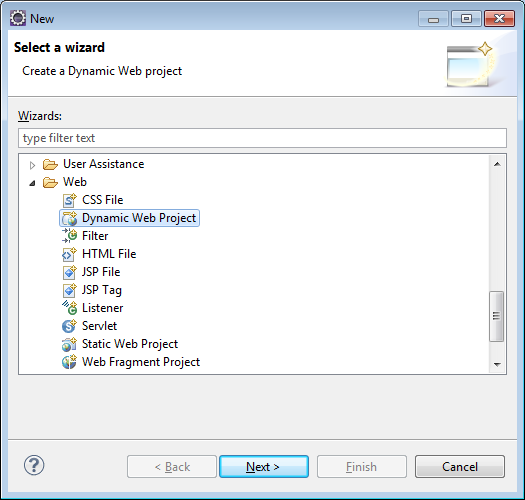
\includegraphics[scale=0.65]{./imagens/apendice_img1.png}}
%   \caption[Exemplo de criação de um projeto Web no Eclipse]
%           {Exemplo de criação de um projeto Web no Eclipse. \textbf{Fonte:} \cite{correa2003plantas}}
% \label{fig:exemplo1}
% \end{figure}
% 
% \par Perceba que o \LaTeX~faz a numeração automática das figuras e já adiciona na lista de figuras.
% 
% \par Agora a mesma imagem foi incluída, porém em escala menhor, conforme ilustra a Figura~\ref{fig:exemplo2}.:
% 
% \begin{figure}[h!]
%   \centerline{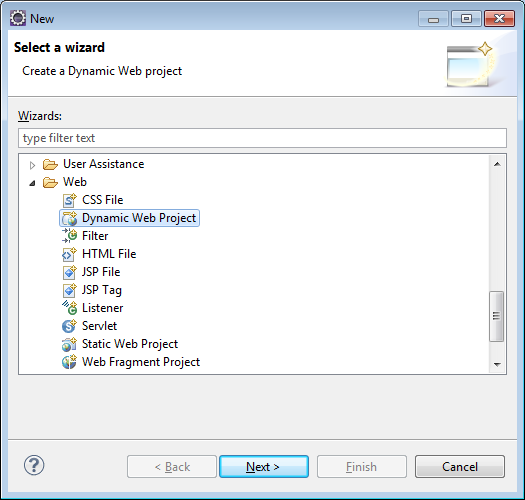
\includegraphics[scale=0.25]{./imagens/apendice_img1.png}}
%   \caption[Mesma imagem em escala menor]
%           {Mesma imagem em escala menor. \textbf{Fonte:} \cite{correa2003plantas}}
% \label{fig:exemplo2}
%\end{figure}



% \par    Desta forma surge a necessidade de primeiramente descrever os
% princípios da teoria proposta por Darwin para que se possa ter um melhor
% entendimento do contexto de computação evolucionária e de algoritmos genéticos.
% É importante, porém, ressaltar que o conteúdo desta sessão não tem como
% objetivo levantar questões sobre o tema da origem dos seres vivos. 
% 	
% \par	O autor afirma ainda que o trabalho de Darwin iniciou-se p
% Esta observação foi o ponto chave que levou o inglês a criar a teoria da evolução. 
% 	
% \par 	Ainda segundo Linden, a teoria afirma que,  

% \par algoritmos genéticos são um ramo de uma das abordagens da inteligência
% artificial denominada abordagem evolutiva. Segundo Lacerda e Carvalho o termo,
% proposto inicialmente por John Holland em 1975 e popularizado através de seu aluno Goldberg
% em 1989, está fundamentado no princípio de seleção natural proposto por Charles Darwin em seu
% livro A Origem das Espécie.
% 
% \par Darwin (1859) propôs que os indivíduos mais fortes evoluem através do processo de
% seleção natural, que define que o indivíduos com melhor capacidade de adaptação ao seu
% ambiente possuem maior chance de sobreviver e gerar descendentes. Algoritmos genéticos
% seguem este mesmo conceito, pois, segundo \citeonline{livro_ags_ricardo_linden},
% são um ramo de um modelo computacional conhecido como algoritmos evolucionários e como tal definem­se como uma
% técnica de otimização e busca que se baseia na teoria do processo de evolução
% natural. \citeonline {livro_ags_ricardo_linden} afirma,
% 
% \begin{citacao}
% “Algoritmos evolucionários funcionam mantendo uma população de estruturas,
% denominadas indivíduos ou cromossomos que se comportam de forma semelhante a
% evolução das espécies. A estas estruturas são aplicados os chamados operadores
% genéticos, como recombinação, mutação, entre outros. Cada indivíduo recebe uma 
% avaliação que é uma quantificaçâo da sua qualidade como solução do problema em
% questão. Com base nesta avaliação serão aplicados os operadores genéticos de forma
% a simular a sobrevivência do mais apto”.\cite[p. 16]{livro_ags_ricardo_linden}
% \end{citacao} 
% 
% \par Técnicas de busca e otimização se destacam pois melhores soluções para um
% problema impacta, muitas vezes, em economia de recursos e neste contexto AGs 
% desempenham um papel importante, pois, como afirma
% \citeonline{nocoes_geriais_anita_fernandes}, “apesar de não garantir que os AGs
% encontrem a solução ótima do problema, existem evidências empíricas de que
% respostas aceitáveis podem ser obtidas em um tempo bastante razoável”.

